%!TEX program = xelatex
\documentclass[11pt,letterpaper]{article}

% ============================================
% MUSCLEMAP FEATURES DOCUMENTATION
% User-Facing Feature Guide
% ============================================

% --- Packages ---
\usepackage[margin=1in]{geometry}
\usepackage{fontspec}
\usepackage{xcolor}
\usepackage{tikz}
\usepackage{pgfplots}
\usepackage{tcolorbox}
\usepackage{fancyhdr}
\usepackage{hyperref}
\usepackage{booktabs}
\usepackage{multicol}
\usepackage{amsmath,amssymb}
\usepackage{fontawesome5}
\usepackage{enumitem}
\usepackage{wrapfig}

% TikZ libraries
\usetikzlibrary{shapes.geometric, arrows.meta, positioning, calc, fit, backgrounds, decorations.pathmorphing, shadows.blur, patterns}

\pgfplotsset{compat=1.18}

% --- Colors ---
\definecolor{mmblue}{HTML}{0066FF}
\definecolor{mmpurple}{HTML}{A855F7}
\definecolor{mmcyan}{HTML}{06B6D4}
\definecolor{mmgreen}{HTML}{22C55E}
\definecolor{mmred}{HTML}{EF4444}
\definecolor{mmyellow}{HTML}{EAB308}
\definecolor{mmpink}{HTML}{EC4899}
\definecolor{mmorange}{HTML}{F97316}
\definecolor{mmvoid}{HTML}{0A0A0F}
\definecolor{mmgray}{HTML}{6B7280}

% Muscle group colors
\definecolor{chestcolor}{HTML}{EF4444}
\definecolor{backcolor}{HTML}{3B82F6}
\definecolor{shouldercolor}{HTML}{F97316}
\definecolor{armcolor}{HTML}{22C55E}
\definecolor{legcolor}{HTML}{A855F7}
\definecolor{corecolor}{HTML}{EAB308}

% --- Fonts ---
\setmainfont{Helvetica Neue}
\setmonofont{Menlo}[Scale=0.9]

% --- Hyperref ---
\hypersetup{
  colorlinks=true,
  linkcolor=mmblue,
  urlcolor=mmpurple,
  pdftitle={MuscleMap Features},
}

% --- Custom Boxes ---
\tcbuselibrary{skins,breakable}

\newtcolorbox{featurebox}[2][]{
  enhanced,
  colback=#2!5,
  colframe=#2!80,
  fonttitle=\bfseries\Large,
  title=#1,
  boxrule=1pt,
  arc=8pt,
  left=12pt,
  right=12pt,
  top=10pt,
  bottom=10pt,
  drop shadow,
}

\newtcolorbox{statbox}[1][]{
  enhanced,
  colback=mmvoid!5,
  colframe=mmcyan!60,
  fonttitle=\bfseries,
  title=#1,
  boxrule=0.5pt,
  arc=4pt,
}

% --- Header/Footer ---
\pagestyle{fancy}
\fancyhf{}
\fancyhead[L]{\textcolor{mmgray}{\small MuscleMap Features}}
\fancyhead[R]{\textcolor{mmgray}{\small User Guide}}
\fancyfoot[C]{\textcolor{mmgray}{\thepage}}
\renewcommand{\headrulewidth}{0.4pt}

% ============================================
% DOCUMENT START
% ============================================
\begin{document}

% --- Title Page ---
\begin{titlepage}
  \centering
  \vspace*{1.5cm}

  % Decorative muscle visualization
  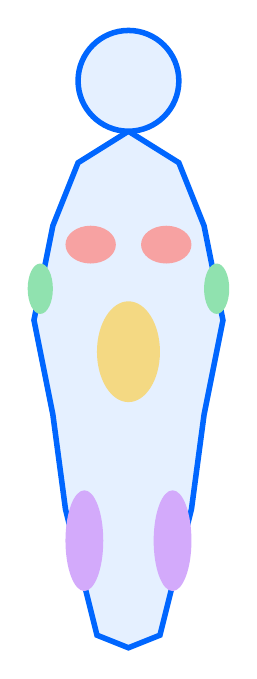
\begin{tikzpicture}[scale=0.8]
    % Body outline (simplified muscular figure)
    \draw[mmblue, line width=2pt, fill=mmblue!10]
      (0,4) -- (0.8,3.5) -- (1.2,2.5) -- (1.5,1) -- (1.2,-0.5) -- (1,-2) -- (0.5,-4) -- (0,-4.2) -- (-0.5,-4) -- (-1,-2) -- (-1.2,-0.5) -- (-1.5,1) -- (-1.2,2.5) -- (-0.8,3.5) -- cycle;

    % Muscle highlights
    \fill[chestcolor!50] (-0.6,2.2) ellipse (0.4 and 0.3);
    \fill[chestcolor!50] (0.6,2.2) ellipse (0.4 and 0.3);
    \fill[armcolor!50] (-1.4,1.5) ellipse (0.2 and 0.4);
    \fill[armcolor!50] (1.4,1.5) ellipse (0.2 and 0.4);
    \fill[corecolor!50] (0,0.5) ellipse (0.5 and 0.8);
    \fill[legcolor!50] (-0.7,-2.5) ellipse (0.3 and 0.8);
    \fill[legcolor!50] (0.7,-2.5) ellipse (0.3 and 0.8);

    % Head
    \draw[mmblue, line width=2pt, fill=mmblue!10] (0,4.8) circle (0.8);
  \end{tikzpicture}

  \vspace{1cm}

  {\Huge\bfseries\textcolor{mmblue}{MuscleMap}\par}
  \vspace{0.3cm}
  {\LARGE\textcolor{mmpurple}{Feature Guide}\par}

  \vspace{1.5cm}

  {\large\textcolor{mmgray}{
    See Every Muscle Fire\\[5pt]
    Track Every Rep\\[5pt]
    Build Your Perfect Physique
  }\par}

  \vfill

  
\begin{tikzpicture}
    % Platform icons
    \foreach \x/\icon/\col in {0/\faGlobe/mmblue, 2/\faMobile/mmpurple, 4/\faClock/mmcyan, 6/\faVrCardboard/mmpink} {
      \node[circle, fill=\col!20, minimum size=1cm] at (\x,0) {\textcolor{\col}{\icon}};
    }
  \end{tikzpicture}

  \vspace{0.5cm}
  {\small\textcolor{mmgray}{Works on Web, iOS, Android, Apple Watch, and Vision Pro}\par}
\end{titlepage}

\tableofcontents
\newpage

% ============================================
% SECTION 1: MUSCLE TRACKING
% ============================================
\section{Real-Time Muscle Tracking}

\begin{featurebox}[\faFire~Muscle Activation Visualization]{mmred}
MuscleMap shows you \textbf{exactly which muscles} you're working during every exercise. Our 3D visualization highlights activated muscles in real-time as you log your sets.
\end{featurebox}

\subsection{Tracked Muscle Groups}

\begin{center}
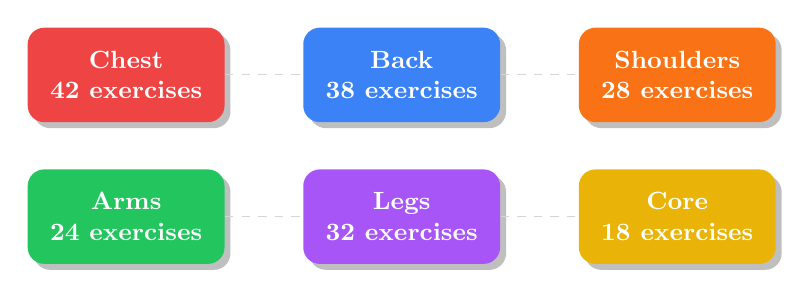
\begin{tikzpicture}[
  muscle/.style={
    rectangle,
    rounded corners=6pt,
    minimum width=2.5cm,
    minimum height=1.2cm,
    align=center,
    font=\small\bfseries,
    text=white,
    drop shadow
  }
]
  % Row 1
  \node[muscle, fill=chestcolor] (chest) at (0,0) {Chest\\42 exercises};
  \node[muscle, fill=backcolor] (back) at (3.5,0) {Back\\38 exercises};
  \node[muscle, fill=shouldercolor] (shoulders) at (7,0) {Shoulders\\28 exercises};

  % Row 2
  \node[muscle, fill=armcolor] (arms) at (0,-1.8) {Arms\\24 exercises};
  \node[muscle, fill=legcolor] (legs) at (3.5,-1.8) {Legs\\32 exercises};
  \node[muscle, fill=corecolor] (core) at (7,-1.8) {Core\\18 exercises};

  % Connecting lines for visual interest
  \draw[mmgray!30, dashed] (chest) -- (back);
  \draw[mmgray!30, dashed] (back) -- (shoulders);
  \draw[mmgray!30, dashed] (arms) -- (legs);
  \draw[mmgray!30, dashed] (legs) -- (core);
\end{tikzpicture}
\end{center}

\subsection{Activation Intensity Scale}

\begin{center}
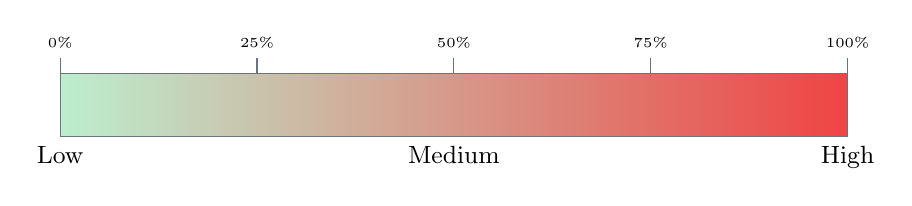
\begin{tikzpicture}
  % Gradient bar
  \shade[left color=mmgreen!30, right color=mmred] (0,0) rectangle (10,0.8);
  \draw[mmgray] (0,0) rectangle (10,0.8);

  % Labels
  \node[below, font=\small] at (0,0) {Low};
  \node[below, font=\small] at (5,0) {Medium};
  \node[below, font=\small] at (10,0) {High};

  % Percentage markers
  \foreach \x/\p in {0/0\%, 2.5/25\%, 5/50\%, 7.5/75\%, 10/100\%} {
    \draw[mmgray] (\x,0.8) -- (\x,1);
    \node[above, font=\tiny] at (\x,1) {\p};
  }
\end{tikzpicture}
\end{center}

% ============================================
% SECTION 2: ARCHETYPES
% ============================================
\section{Training Archetypes}

Choose your training style and unlock specialized progression paths:

\begin{center}
\begin{tikzpicture}[
  archetype/.style={
    rectangle,
    rounded corners=8pt,
    draw=#1,
    fill=#1!10,
    minimum width=3cm,
    minimum height=2cm,
    align=center,
    font=\small
  }
]
  % Row 1
  \node[archetype=mmred] (bodybuilder) at (0,0) {\faUser\\[3pt]\textbf{Bodybuilder}\\Hypertrophy Focus};
  \node[archetype=mmblue] (powerlifter) at (4,0) {\faDumbbell\\[3pt]\textbf{Powerlifter}\\Strength Focus};
  \node[archetype=mmgreen] (athlete) at (8,0) {\faRunning\\[3pt]\textbf{Athlete}\\Performance};
  \node[archetype=mmpurple] (gymnast) at (12,0) {\faChild\\[3pt]\textbf{Gymnast}\\Calisthenics};

  % Row 2
  \node[archetype=mmorange] (crossfit) at (0,-3) {\faFire\\[3pt]\textbf{CrossFit}\\Functional};
  \node[archetype=mmcyan] (martial) at (4,-3) {\faHandRock\\[3pt]\textbf{Martial Artist}\\Combat Sports};
  \node[archetype=mmpink] (yoga) at (8,-3) {\faSpa\\[3pt]\textbf{Yogi}\\Flexibility};
  \node[archetype=mmyellow] (runner) at (12,-3) {\faRunning\\[3pt]\textbf{Runner}\\Endurance};
\end{tikzpicture}
\end{center}

\subsection{Archetype Distribution}

\begin{center}
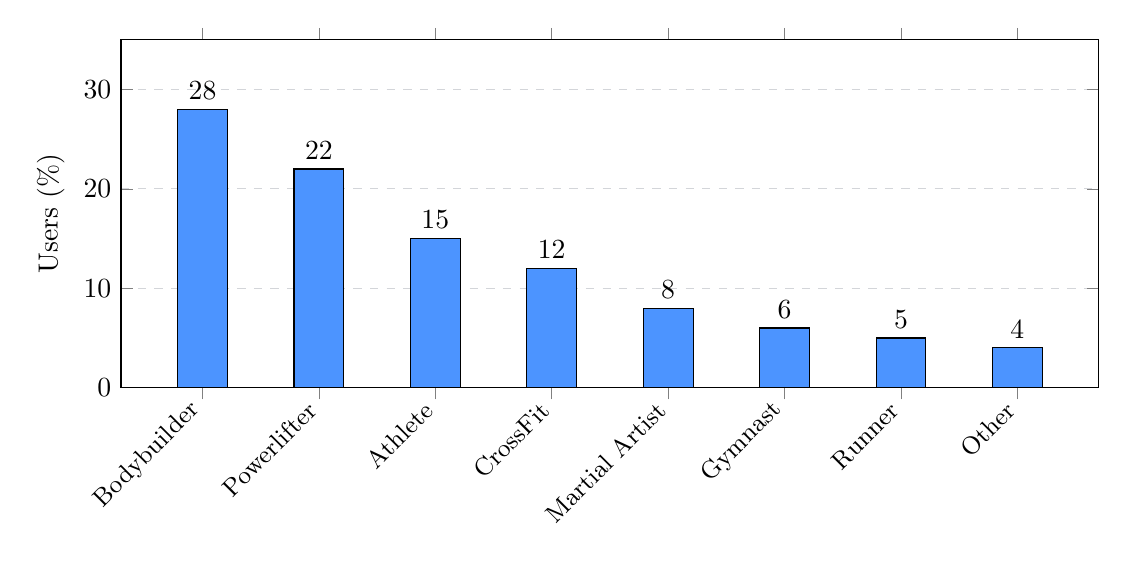
\begin{tikzpicture}
\begin{axis}[
  ybar,
  bar width=18pt,
  width=14cm,
  height=6cm,
  ylabel={Users (\%)},
  symbolic x coords={Bodybuilder, Powerlifter, Athlete, CrossFit, Martial Artist, Gymnast, Runner, Other},
  xtick=data,
  x tick label style={rotate=45, anchor=east, font=\small},
  nodes near coords,
  nodes near coords align={vertical},
  ymin=0,
  ymax=35,
  ymajorgrids=true,
  grid style={dashed, mmgray!30},
]
\addplot[fill=mmblue!70] coordinates {
  (Bodybuilder, 28)
  (Powerlifter, 22)
  (Athlete, 15)
  (CrossFit, 12)
  (Martial Artist, 8)
  (Gymnast, 6)
  (Runner, 5)
  (Other, 4)
};
\end{axis}
\end{tikzpicture}
\end{center}

% ============================================
% SECTION 3: PROGRESSION SYSTEM
% ============================================
\section{RPG-Style Progression}

\begin{featurebox}[\faChartLine~Level Up Your Character]{mmpurple}
MuscleMap gamifies your fitness journey with an RPG-inspired progression system. Earn XP, level up, and watch your character stats grow!
\end{featurebox}

\subsection{Character Stats}

\begin{center}
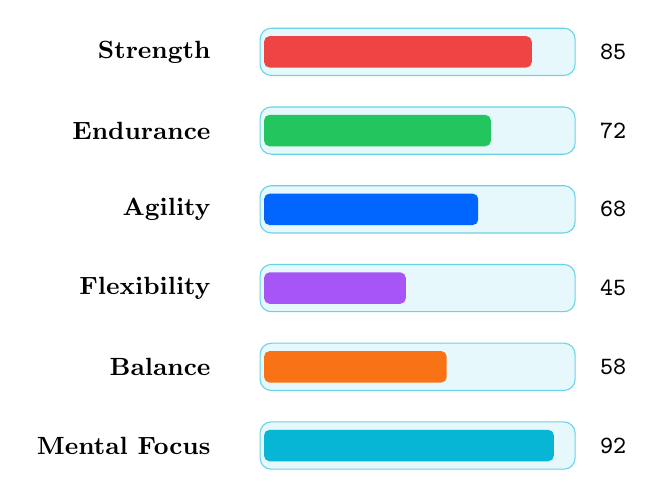
\begin{tikzpicture}[
  stat/.style={
    rectangle,
    rounded corners=4pt,
    draw=mmcyan!60,
    fill=mmcyan!10,
    minimum width=4cm,
    minimum height=0.6cm,
    font=\small
  },
  bar/.style={
    rectangle,
    rounded corners=2pt,
    minimum height=0.4cm
  }
]
  % Stats list - manually placed to avoid foreach parsing issues
  \node[anchor=east, font=\small\bfseries] at (-0.5,0) {Strength};
  \node[stat, anchor=west] at (0,0) {};
  \node[bar, fill=mmred, minimum width=3.4cm, anchor=west] at (0.05,0) {};
  \node[anchor=west, font=\small\ttfamily] at (4.2,0) {85};

  \node[anchor=east, font=\small\bfseries] at (-0.5,-1) {Endurance};
  \node[stat, anchor=west] at (0,-1) {};
  \node[bar, fill=mmgreen, minimum width=2.88cm, anchor=west] at (0.05,-1) {};
  \node[anchor=west, font=\small\ttfamily] at (4.2,-1) {72};

  \node[anchor=east, font=\small\bfseries] at (-0.5,-2) {Agility};
  \node[stat, anchor=west] at (0,-2) {};
  \node[bar, fill=mmblue, minimum width=2.72cm, anchor=west] at (0.05,-2) {};
  \node[anchor=west, font=\small\ttfamily] at (4.2,-2) {68};

  \node[anchor=east, font=\small\bfseries] at (-0.5,-3) {Flexibility};
  \node[stat, anchor=west] at (0,-3) {};
  \node[bar, fill=mmpurple, minimum width=1.8cm, anchor=west] at (0.05,-3) {};
  \node[anchor=west, font=\small\ttfamily] at (4.2,-3) {45};

  \node[anchor=east, font=\small\bfseries] at (-0.5,-4) {Balance};
  \node[stat, anchor=west] at (0,-4) {};
  \node[bar, fill=mmorange, minimum width=2.32cm, anchor=west] at (0.05,-4) {};
  \node[anchor=west, font=\small\ttfamily] at (4.2,-4) {58};

  \node[anchor=east, font=\small\bfseries] at (-0.5,-5) {Mental Focus};
  \node[stat, anchor=west] at (0,-5) {};
  \node[bar, fill=mmcyan, minimum width=3.68cm, anchor=west] at (0.05,-5) {};
  \node[anchor=west, font=\small\ttfamily] at (4.2,-5) {92};
\end{tikzpicture}
\end{center}

\subsection{XP \& Leveling Formula}

The experience required for each level follows a diminishing returns curve:

\begin{equation*}
\text{XP}_{\text{required}}(L) = \left\lfloor 100 \times L^{1.5} \right\rfloor
\end{equation*}

\begin{center}
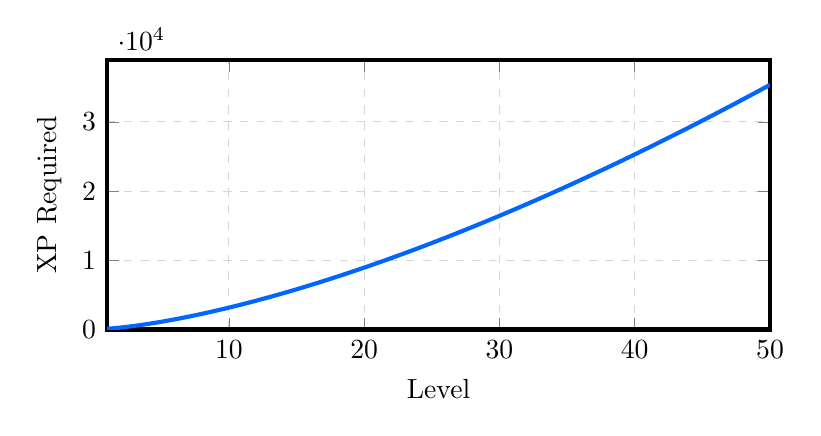
\begin{tikzpicture}
\begin{axis}[
  width=10cm,
  height=5cm,
  xlabel={Level},
  ylabel={XP Required},
  xmin=1, xmax=50,
  ymin=0,
  grid=major,
  grid style={dashed, mmgray!30},
  line width=1.5pt,
]
\addplot[mmblue, smooth, domain=1:50, samples=50] {100*x^1.5};
\end{axis}
\end{tikzpicture}
\end{center}

% ============================================
% SECTION 4: CROSS-PLATFORM
% ============================================
\section{Cross-Platform Experience}

\begin{center}
\begin{tikzpicture}[
  device/.style={
    rectangle,
    rounded corners=10pt,
    draw=#1,
    fill=#1!10,
    minimum width=3cm,
    minimum height=4cm,
    align=center
  },
  screen/.style={
    rectangle,
    rounded corners=4pt,
    fill=mmvoid,
    minimum width=2.4cm,
    minimum height=2.8cm
  }
]
  % Web Browser
  \node[device=mmblue] (web) at (0,0) {};
  \node[screen] at (0,0.3) {};
  \node[above, font=\small\bfseries, mmblue] at (0,2.2) {Web Browser};
  \node[below, font=\tiny, mmgray] at (0,-2.2) {Chrome, Safari, Firefox};
  \node[white, font=\large] at (0,0.3) {\faGlobe};

  % Mobile
  \node[device=mmpurple] (mobile) at (4.5,0) {};
  \node[screen, minimum width=2cm, minimum height=2.6cm] at (4.5,0.3) {};
  \node[above, font=\small\bfseries, mmpurple] at (4.5,2.2) {Mobile Apps};
  \node[below, font=\tiny, mmgray] at (4.5,-2.2) {iOS \& Android};
  \node[white, font=\large] at (4.5,0.3) {\faMobile};

  % Watch
  \node[device=mmcyan, minimum width=2.5cm, minimum height=3cm] (watch) at (8.5,0) {};
  \node[screen, minimum width=1.8cm, minimum height=1.8cm] at (8.5,0.2) {};
  \node[above, font=\small\bfseries, mmcyan] at (8.5,1.7) {Apple Watch};
  \node[below, font=\tiny, mmgray] at (8.5,-1.7) {Wrist tracking};
  \node[white, font=\large] at (8.5,0.2) {\faClock};

  % Vision Pro
  \node[device=mmpink, minimum width=3.5cm, minimum height=2.5cm] (vision) at (12.5,0) {};
  \node[screen, minimum width=3cm, minimum height=1.5cm, rounded corners=8pt] at (12.5,0.2) {};
  \node[above, font=\small\bfseries, mmpink] at (12.5,1.5) {Vision Pro};
  \node[below, font=\tiny, mmgray] at (12.5,-1.5) {Spatial computing};
  \node[white, font=\large] at (12.5,0.2) {\faVrCardboard};

  % Sync arrows
  \draw[->, mmgreen, line width=2pt, dashed] (1.8,0) -- (2.7,0);
  \draw[->, mmgreen, line width=2pt, dashed] (6.3,0) -- (7.2,0);
  \draw[->, mmgreen, line width=2pt, dashed] (9.8,0) -- (10.7,0);

  % Sync label
  \node[font=\scriptsize, mmgreen] at (6.5,-3) {\faSync~Real-time sync across all devices};
\end{tikzpicture}
\end{center}

% ============================================
% SECTION 5: WEARABLES
% ============================================
\section{Wearable Integrations}

\begin{statbox}[Supported Devices]
\begin{center}
\begin{tabular}{@{}lcl@{}}
\toprule
\textbf{Device} & \textbf{Status} & \textbf{Data Synced} \\
\midrule
Apple HealthKit & \textcolor{mmgreen}{\faCheckCircle} & HR, Workouts, Steps \\
Google Fit & \textcolor{mmgreen}{\faCheckCircle} & HR, Workouts, Steps \\
Apple Watch & \textcolor{mmgreen}{\faCheckCircle} & Real-time HR, Calories \\
Fitbit & \textcolor{mmgreen}{\faCheckCircle} & Sleep, HR, Activity \\
Oura Ring & \textcolor{mmgreen}{\faCheckCircle} & Sleep, Recovery \\
Garmin Connect & \textcolor{mmyellow}{\faClock} & Coming Soon \\
Whoop & \textcolor{mmyellow}{\faClock} & Coming Soon \\
\bottomrule
\end{tabular}
\end{center}
\end{statbox}

% ============================================
% SECTION 6: SOCIAL FEATURES
% ============================================
\section{Community \& Social}

\begin{multicols}{2}

\subsection{High Fives}
Send encouragement to other athletes with our ``High Five'' system. Boost motivation and build connections.

\begin{center}
\begin{tikzpicture}
  \node[circle, fill=mmyellow!30, minimum size=2cm] {\textcolor{mmyellow}{\Huge\faHandPaper}};
\end{tikzpicture}
\end{center}

\columnbreak

\subsection{Leaderboards}
Compete globally or within your region. See where you rank across:
\begin{itemize}
  \item Total Training Units (TU)
  \item Workout Streaks
  \item Archetype Rankings
  \item Monthly Challenges
\end{itemize}

\end{multicols}

\subsection{Crews}

Form or join a \textbf{Crew} to train together, compete in crew wars, and share achievements.

\begin{center}
\begin{tikzpicture}[
  member/.style={circle, fill=mmblue!20, minimum size=1cm, font=\small}
]
  % Crew circle
  \node[circle, draw=mmpurple, line width=2pt, minimum size=4cm, fill=mmpurple!5] (crew) {};
  \node[below, mmpurple, font=\bfseries] at (crew.south) {Your Crew};

  % Members
  \node[member] at (0,1) {\faUser};
  \node[member] at (1,0) {\faUser};
  \node[member] at (0.5,-0.8) {\faUser};
  \node[member] at (-0.7,0.3) {\faUser};
  \node[member] at (-0.3,-0.5) {\faStar};
\end{tikzpicture}
\end{center}

% ============================================
% SECTION 7: AI FEATURES
% ============================================
\section{AI-Powered Features}

\begin{featurebox}[\faRobot~Smart Workout Generation]{mmcyan}
Our AI analyzes your goals, available equipment, and training history to generate personalized workout plans tailored to your archetype.
\end{featurebox}

\subsection{How It Works}

\begin{center}
\begin{tikzpicture}[
  step/.style={
    rectangle,
    rounded corners=6pt,
    draw=mmcyan,
    fill=mmcyan!10,
    minimum width=2.5cm,
    minimum height=1.5cm,
    align=center,
    font=\small
  },
  arrow/.style={->, >=Stealth, line width=2pt, mmcyan}
]
  \node[step] (input) at (0,0) {\faEdit\\[3pt]Enter Goals\\Equipment};
  \node[step] (ai) at (4.5,0) {\faBrain\\[3pt]AI Analysis\\Optimization};
  \node[step] (output) at (9,0) {\faClipboardList\\[3pt]Personalized\\Workout};

  \draw[arrow] (input) -- (ai);
  \draw[arrow] (ai) -- (output);
\end{tikzpicture}
\end{center}

% ============================================
% GETTING STARTED
% ============================================
\section{Getting Started}

\begin{enumerate}[leftmargin=*]
  \item \textbf{Create Account} --- Sign up at \url{https://musclemap.me}
  \item \textbf{Choose Archetype} --- Select your training style
  \item \textbf{Set Goals} --- Define what you want to achieve
  \item \textbf{Connect Devices} --- Link your wearables (optional)
  \item \textbf{Start Training} --- Log workouts and watch your progress!
\end{enumerate}

\begin{center}
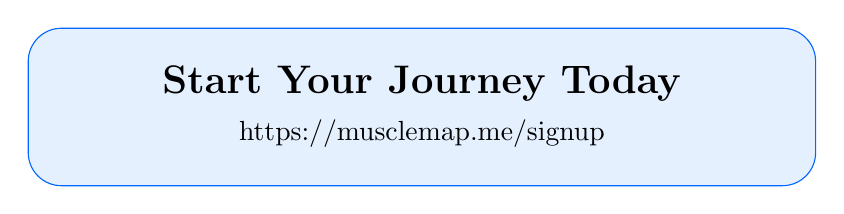
\begin{tikzpicture}
\node[
  rectangle,
  rounded corners=12pt,
  draw=mmblue,
  fill=mmblue!10,
  minimum width=10cm,
  minimum height=2cm,
  align=center
] {
  \textbf{\Large Start Your Journey Today}\\[5pt]
  \url{https://musclemap.me/signup}
};
\end{tikzpicture}
\end{center}

\end{document}
